% Options for packages loaded elsewhere
\PassOptionsToPackage{unicode}{hyperref}
\PassOptionsToPackage{hyphens}{url}
\PassOptionsToPackage{dvipsnames,svgnames,x11names}{xcolor}
%
\documentclass[
]{article}

\usepackage{amsmath,amssymb}
\usepackage{iftex}
\ifPDFTeX
  \usepackage[T1]{fontenc}
  \usepackage[utf8]{inputenc}
  \usepackage{textcomp} % provide euro and other symbols
\else % if luatex or xetex
  \usepackage{unicode-math}
  \defaultfontfeatures{Scale=MatchLowercase}
  \defaultfontfeatures[\rmfamily]{Ligatures=TeX,Scale=1}
\fi
\usepackage{lmodern}
\ifPDFTeX\else  
    % xetex/luatex font selection
  \setmainfont[]{Latin Modern Roman}
  \setmathfont[]{Latin Modern Math}
\fi
% Use upquote if available, for straight quotes in verbatim environments
\IfFileExists{upquote.sty}{\usepackage{upquote}}{}
\IfFileExists{microtype.sty}{% use microtype if available
  \usepackage[]{microtype}
  \UseMicrotypeSet[protrusion]{basicmath} % disable protrusion for tt fonts
}{}
\makeatletter
\@ifundefined{KOMAClassName}{% if non-KOMA class
  \IfFileExists{parskip.sty}{%
    \usepackage{parskip}
  }{% else
    \setlength{\parindent}{0pt}
    \setlength{\parskip}{6pt plus 2pt minus 1pt}}
}{% if KOMA class
  \KOMAoptions{parskip=half}}
\makeatother
\usepackage{xcolor}
\setlength{\emergencystretch}{3em} % prevent overfull lines
\setcounter{secnumdepth}{5}
% Make \paragraph and \subparagraph free-standing
\ifx\paragraph\undefined\else
  \let\oldparagraph\paragraph
  \renewcommand{\paragraph}[1]{\oldparagraph{#1}\mbox{}}
\fi
\ifx\subparagraph\undefined\else
  \let\oldsubparagraph\subparagraph
  \renewcommand{\subparagraph}[1]{\oldsubparagraph{#1}\mbox{}}
\fi


\providecommand{\tightlist}{%
  \setlength{\itemsep}{0pt}\setlength{\parskip}{0pt}}\usepackage{longtable,booktabs,array}
\usepackage{calc} % for calculating minipage widths
% Correct order of tables after \paragraph or \subparagraph
\usepackage{etoolbox}
\makeatletter
\patchcmd\longtable{\par}{\if@noskipsec\mbox{}\fi\par}{}{}
\makeatother
% Allow footnotes in longtable head/foot
\IfFileExists{footnotehyper.sty}{\usepackage{footnotehyper}}{\usepackage{footnote}}
\makesavenoteenv{longtable}
\usepackage{graphicx}
\makeatletter
\def\maxwidth{\ifdim\Gin@nat@width>\linewidth\linewidth\else\Gin@nat@width\fi}
\def\maxheight{\ifdim\Gin@nat@height>\textheight\textheight\else\Gin@nat@height\fi}
\makeatother
% Scale images if necessary, so that they will not overflow the page
% margins by default, and it is still possible to overwrite the defaults
% using explicit options in \includegraphics[width, height, ...]{}
\setkeys{Gin}{width=\maxwidth,height=\maxheight,keepaspectratio}
% Set default figure placement to htbp
\makeatletter
\def\fps@figure{htbp}
\makeatother
% definitions for citeproc citations
\NewDocumentCommand\citeproctext{}{}
\NewDocumentCommand\citeproc{mm}{%
  \begingroup\def\citeproctext{#2}\cite{#1}\endgroup}
\makeatletter
 % allow citations to break across lines
 \let\@cite@ofmt\@firstofone
 % avoid brackets around text for \cite:
 \def\@biblabel#1{}
 \def\@cite#1#2{{#1\if@tempswa , #2\fi}}
\makeatother
\newlength{\cslhangindent}
\setlength{\cslhangindent}{1.5em}
\newlength{\csllabelwidth}
\setlength{\csllabelwidth}{3em}
\newenvironment{CSLReferences}[2] % #1 hanging-indent, #2 entry-spacing
 {\begin{list}{}{%
  \setlength{\itemindent}{0pt}
  \setlength{\leftmargin}{0pt}
  \setlength{\parsep}{0pt}
  % turn on hanging indent if param 1 is 1
  \ifodd #1
   \setlength{\leftmargin}{\cslhangindent}
   \setlength{\itemindent}{-1\cslhangindent}
  \fi
  % set entry spacing
  \setlength{\itemsep}{#2\baselineskip}}}
 {\end{list}}
\usepackage{calc}
\newcommand{\CSLBlock}[1]{\hfill\break\parbox[t]{\linewidth}{\strut\ignorespaces#1\strut}}
\newcommand{\CSLLeftMargin}[1]{\parbox[t]{\csllabelwidth}{\strut#1\strut}}
\newcommand{\CSLRightInline}[1]{\parbox[t]{\linewidth - \csllabelwidth}{\strut#1\strut}}
\newcommand{\CSLIndent}[1]{\hspace{\cslhangindent}#1}

\usepackage{booktabs}
\usepackage{caption}
\usepackage{longtable}
\usepackage{colortbl}
\usepackage{array}
\usepackage{tipa}
\usepackage{booktabs}
\usepackage{arxiv}
\usepackage{orcidlink}
\usepackage{amsmath}
\usepackage[T1]{fontenc}
\makeatletter
\@ifpackageloaded{caption}{}{\usepackage{caption}}
\AtBeginDocument{%
\ifdefined\contentsname
  \renewcommand*\contentsname{Table of contents}
\else
  \newcommand\contentsname{Table of contents}
\fi
\ifdefined\listfigurename
  \renewcommand*\listfigurename{List of Figures}
\else
  \newcommand\listfigurename{List of Figures}
\fi
\ifdefined\listtablename
  \renewcommand*\listtablename{List of Tables}
\else
  \newcommand\listtablename{List of Tables}
\fi
\ifdefined\figurename
  \renewcommand*\figurename{Figure}
\else
  \newcommand\figurename{Figure}
\fi
\ifdefined\tablename
  \renewcommand*\tablename{Table}
\else
  \newcommand\tablename{Table}
\fi
}
\@ifpackageloaded{float}{}{\usepackage{float}}
\floatstyle{ruled}
\@ifundefined{c@chapter}{\newfloat{codelisting}{h}{lop}}{\newfloat{codelisting}{h}{lop}[chapter]}
\floatname{codelisting}{Listing}
\newcommand*\listoflistings{\listof{codelisting}{List of Listings}}
\makeatother
\makeatletter
\makeatother
\makeatletter
\@ifpackageloaded{caption}{}{\usepackage{caption}}
\@ifpackageloaded{subcaption}{}{\usepackage{subcaption}}
\makeatother
\ifLuaTeX
\usepackage[bidi=basic]{babel}
\else
\usepackage[bidi=default]{babel}
\fi
\babelprovide[main,import]{english}
\ifPDFTeX
\else
\babelfont{rm}[]{Latin Modern Roman}
\fi
% get rid of language-specific shorthands (see #6817):
\let\LanguageShortHands\languageshorthands
\def\languageshorthands#1{}
\ifLuaTeX
  \usepackage{selnolig}  % disable illegal ligatures
\fi
\usepackage{bookmark}

\IfFileExists{xurl.sty}{\usepackage{xurl}}{} % add URL line breaks if available
\urlstyle{same} % disable monospaced font for URLs
\hypersetup{
  pdftitle={The role of cognateness in non-native spoken word recognition},
  pdfauthor={Gonzalo Garcia-Castro; Serene Siow; Kim Plunkett; Nuria Sebastian-Galles},
  pdflang={en},
  pdfkeywords={cognate, spoken word
recognition, phonology, bilingualism, non-native speech
processing, lexical access},
  colorlinks=true,
  linkcolor={blue},
  filecolor={Maroon},
  citecolor={Blue},
  urlcolor={Blue},
  pdfcreator={LaTeX via pandoc}}

\usepackage{lineno}
\linenumbers
\newcommand{\runninghead}{A Preprint }
\renewcommand{\runninghead}{Cognateness and non-native word
recognition }
\title{The role of cognateness in non-native spoken word recognition}
\author{\textbf{Gonzalo
Garcia-Castro}~\orcidlink{0000-0002-8553-4209}\\Center for Brain and
Cognition\\Universitat Pompeu Fabra\\Barcelona,
08005\\\texttt{\href{mailto:gonzalo.garciadecastro@upf.edu}{gonzalo.garciadecastro@upf.edu}}\And\textbf{Serene
Siow}~\orcidlink{0000-0001-6482-2191}\\Department of Experimental
Psychology\\University of Oxford\\Oxford, OX2
6GG\\\texttt{\href{mailto:siow.serene@gmail.com}{siow.serene@gmail.com}}\And\textbf{Kim
Plunkett}~\orcidlink{0000-0003-0216-7480}\\Department of Experimental
Psychology\\University of Oxford\\Oxford, OX2
6GG\\\texttt{\href{mailto:kim.plunkett@psy.ox.ac.uk}{kim.plunkett@psy.ox.ac.uk}}\And\textbf{Nuria
Sebastian-Galles}~\orcidlink{0000-0001-6938-2498}\\Center for Brain and
Cognition\\Universitat Pompeu Fabra\\Barcelona,
08005\\\texttt{\href{mailto:nuria.sebastian@upf.edu}{nuria.sebastian@upf.edu}}}
\date{}
\begin{document}
\maketitle
\begin{abstract}
Understanding spoken words in a non-native language is easier when the
words are phonologically similar to their translations into the
listener's native language are phonologically similar. Phonological
similarity plays a more important role in the language performance of
low-proficiency bilinguals, compared to that of high-proficiency
bilinguals., and This suggests that low-proficiency bilinguals may
points to the latter as relying more strongly on cross-language
word-to-word links (lexical route), while high-proficiency bilinguals
rely more on word-concept associations (conceptual route) than on
cross-language word-to-word links (lexical route). Disentangling
bilinguals' reliance on the conceptual and lexical and conceptual routes
during translation is challenging, given that both sources of
information are present during spoken word comprehensionto some extent
in both high- and low-proficiency bilinguals. In this study, we tested
English and Spanish native speakers in a translation elicitation task,
in which they listened to words in an unfamiliar language (Spanish or
Catalan for English natives, and Catalan for Spanish natives), and then
had to translate them to their native language. Given their lack of
previous knowledge ion the unfamiliar tested language, phonological
similarity between the presented words and their correct translations
was the only cue available for participants to succeed in the task. This
allowed us to explore the informativeness of the lexical route for word
translation, in the absence of information from the conceptual route.
Our results indicate that participants benefited from the phonological
similarity between translation equivalents: the more similar the word
they listened to and its translational equivalent, the higher the
probability of a correct translation. These results point to
cross-language word-to-word links as providing rich information during
word translation.
\end{abstract}
{\bfseries \emph Keywords}
\def\sep{\textbullet\ }
cognate \sep spoken word
recognition \sep phonology \sep bilingualism \sep non-native speech
processing \sep 
lexical access


\section{Introduction}\label{introduction}

Listening to non-native speech is costlier than listening to native
speech, even for highly proficient bilinguals, and especially in
acoustically adverse situations
(\citeproc{ref-lecumberri2010non}{Lecumberri et al., 2010};
\citeproc{ref-takata1990english}{Takata \& Nábělek, 1990}). However,
there are some sources of information which may make non-native speech
comprehension easier. One of the sources of this increased difficulty
stems from the possible mismatch between the phonology of the native and
the non-native languages: some acoustic features embedded in the
non-native speech signal do not overlap perfectly with any phonemic
category in the listener's native language. For example, imagine a
Spanish native, with no previous familiarity with any other language,
who listens for the first time to French may encounter the word /pɔʁt/
(\emph{porte}), translation of door in French. The voiced uvular
fricative consonant /ʁ/ and the open-mid back rounded vowel /ɔ/ do not
exist in Spanish as phonemic categories. These discrepancies can
nonetheless be perceived as allophonic variations the native (Spanish)
phonemes /r/ and /o/ (\citeproc{ref-best2001discrimination}{Best et al.,
2001}), and the non-native speech signal may engage lexical processing
mechanisms (\citeproc{ref-weber2004lexical}{Weber \& Cutler, 2004}),
leading to the activation and selection, and therefore the recognition
of its translation to Spanish /ˈpwer.ta/ (\emph{puerta}). The
recognition of this French, unfamiliar word relies almost entirely on
its similarity with its Spanish translation. Conversely, imagine now
that the same Spanish listener hears English for the first time and
encounters the word /dɔː/ (\emph{door}). This time, phonological
similarity is of little help: /ˈpwer.ta/ and /dɔː/ share very few
phonemes. It would come as a surprise if the listener was able to
translate the English word successfully, if not by relying on previously
learnt word-concept associations (which they lack, as they are
unfamiliar to English).

Cross-language phonological similarity seems, at face value, an
important source of information for unfamiliar listeners during auditory
word recognition, even if translations are not phonologically identical.
Although this mismatch has a noticeable toll on comprehension
(\citeproc{ref-cutler2004patterns}{Cutler et al., 2004}), the fact that
word recognition can take place at all in such circumstances illustrates
that non-native listeners--even low-proficiency ones--are rarely
completely naïve to the language they are listening to. In the present
study, we investigate the extent to which adult listeners rely on the
phonological similarity between their native and non-native languages
during word recognition, capitalising on the role of \emph{cognates.}

Many languages share, to some extent, similarities at the lexical level.
This is frequently due to their typological closeness and/or
socio-historical events involving the speakers of these languages (e.g.,
migration, social contact). Cognates embody a particular case of such
commonalities. Cognates are defined as cross-language synonyms which
have similar forms whose form is similar (at the phonological level,
orthographic level, signed level), commonly due to their shared
etymological origin\footnote{Some form-similar cross-language synonyms
  are technically not cognates. For example, \emph{sun} and \emph{sol}
  (in Spanish) share phonological onset but their etymology points to
  different origins. The complimentary case is equally problematic when
  defining cognateness: cross-language synonyms that share etymological
  origin may not be necessarily be recognised as cognates by the average
  listener. Such is the case of \emph{cheese} and \emph{queso} which
  share Latin root but are phonologically dissimilar. For simplicity, we
  will use the term \emph{cognateness} in this paper to include all
  cross-language synonyms that fulfill a specified threshold of form
  similarity, regardless of etymology. We do not expect that etymology
  plays a direct role on language perception if it is not via
  form-similarity, since it is not necessary for participants in
  psycholinguistic experiments to be aware of the etymology of the words
  they encounter in the tasks to be subject to the effect of
  form-similarity.}. For example, Romance languages such as Spanish and
Catalan share many cognates
(\citeproc{ref-schepens2012distributions}{Schepens et al., 2012}), as in
the case of \emph{puerta} and \emph{porta} (door in Spanish and Catalan,
respectively). Cognates play a pivotal role in many models of bilingual
lexical processing because they provide evidence that bilinguals access
the lexicon in a language non-selective way. For instance, pictures are
named faster by Spanish-Catalan bilinguals when their associated labels
in both languages are cognates (e.g., \emph{puerta}-\emph{porta}),
compared to when their labels are non-cognates
(\emph{mesa}-\emph{taula}, {[}table{]}), which suggests that word
representations of both languages are activated during word retrieval
(\citeproc{ref-costa2000cognate}{Costa et al., 2000}). This cognate
advantage is not restricted to production, but also extends to word
recognition (\citeproc{ref-midgley2011effects}{Midgley et al., 2011};
\citeproc{ref-thierry2007brain}{Thierry \& Wu, 2007}), word learning
(\citeproc{ref-de2000hard}{De Groot \& Keijzer, 2000};
\citeproc{ref-elias2022cross}{Elias \& Degani, 2022};
\citeproc{ref-lotto1998effects}{Lotto \& De Groot, 1998};
\citeproc{ref-valente2018does}{Valente et al., 2018}), and word
translation (\citeproc{ref-christoffels2006memory}{Christoffels et al.,
2006}).

\subsection{Lexical and conceptual routes for
translation}\label{lexical-and-conceptual-routes-for-translation}

Early theoretical accounts of this `Cognate effect' proposed that the
impact of cognateness on lexical processing depends on bilinguals'
proficiency in their second language (L2)
(\citeproc{ref-potter1984lexical}{Potter et al., 1984}; see
\citeproc{ref-chen1989patterns}{Chen \& Leung, 1989} for similar
results). The reasoning behind this claim was the assumption that
second-language learners start acquiring words in their L2 by
associating them to their translation in their L1 (lexical route),
instead of directly to their shared concept (conceptual route). This
word-to-word connectivity should be sensitive to form-similarity (i.e.,
cognateness): the more similar the two word- forms are, the stronger the
connection. As learners become more proficient, the connection between
L2 representations and their meaning grows stronger, and L2 word
processing becomes less reliant on word-word connections between L1 and
L2 representations. Cognates subsequently exert less impact on lexical
processing in proficient speakers (see
\citeproc{ref-andras2022cognate}{Andras et al., 2022} for recent
experimental evidence for this claim). The Revised Hierarchical Model
(RHM, \citeproc{ref-kroll1994category}{Kroll \& Stewart, 1994}) captured
this hypothesis and predicted that translating words from L1 to L2
should take longer than translating from L2 to L1. The rationale behind
this prediction was that L1-to-L2 translation relies more strongly on
word-to-word links between L1 and L2 representations, where L2-to-L1
translation relies more strongly on the mediation between the concept
and the two word- forms. L1-to-L2 translation should therefore be more
sensitive to the form similarity between the L1 and the L2
representations: cognate words should be retrieved faster than
non-cognate words during L1-to-L2 translation.

To test these predictions, Groot et al.
(\citeproc{ref-degroot1994forward}{1994}) and Groot
(\citeproc{ref-de1992determinants}{1992}) asked Dutch natives with high
(but non-native) English proficiency to translate Dutch words to English
(L1-to-L2) or English words to Dutch (L2-to-L1). Although participants'
performance in both conditions was roughly equivalent for cognates,
non-cognates were translated more slowly from Dutch to English than from
English to Dutch, suggesting that L1-to-L2 translation is more sensitive
to form-similarity than L2-to-L1 translation. Conversely, participants'
performance was more sensitive to semantic variables (e.g.,
concreteness) when translating English words to Dutch, compared to when
translating Dutch words to English, suggesting that L2-to-L1 translation
was more sensitive to the shared conceptual properties of the
translation pair.

These findings support a soft version of the RHM model, in which both
the conceptual and the lexical translation routes are active during
translation, but where L1-to-L2 translation relies more strongly on
word-to-word links between L1 and L2 representations than L2-to-L1
translation does, and therefore is more sensitive to cognateness.
Further evidence for the presence of this difference between L1-to-L2
and L2-to-L1 translations on the degree of reliance on the lexical and
or the conceptual routes between L1-to-L2 and L2-to-L1 translation was
provided by Phillips et al. (\citeproc{ref-phillips2006erp}{2006}), who
used eletrophysiological recordings of bilinguals translating words from
L1 to L2 or \emph{vice versa} after semantic or phonological priming.
The authors reported stronger N400 responses (associated with semantic
priming) in L1-to-L2 translation than in L2-to-L12 translation, and
stronger phonological mismatch negativity responses (associated with
phonological priming) during L2-to-L1 translation, compared to L1-to-L2
translation.

\subsection{Competition from lexical
neighbours}\label{competition-from-lexical-neighbours}

Since the RHM model was proposed, later studies on monolingual
populations have focused how on the role of the network of connections
that words establish networks of connections with each other at the
form-level (phonological or orthographic) or at the conceptual level.
For instance, the Neighbourhood Activation Model (NAM,
\citeproc{ref-luce1998recognizing}{Luce \& Pisoni, 1998}) highlighted
how lexical selection is affected by the number of phonological
neighbours that the selected word has. Words surrounded by a larger
number of phonological neighbours (words that only differ in one phoneme
from the target word) are responded to more slowly and less accurately
than words from sparser phonological neighbourhoods
(\citeproc{ref-goldinger1989priming}{Goldinger et al., 1989};
\citeproc{ref-luce1990similarity}{Luce et al., 1990}), especially when
these neighbours' lexical frequency is higher
(\citeproc{ref-luce1998recognizing}{Luce \& Pisoni, 1998}).

The existence of phonological links between words is supported with
experimental evidence from the visual world paradigm and phonological
priming. Meyer \& Damian (\citeproc{ref-meyer2007activation}{2007})
showed that target pictures were named faster when presented together
with a phonologically-related distractor, suggesting that the activation
of shared phonological information allowed the target to be activated
and produced faster. there are also findings suggesting that
facilitatory or inhibitory effects on target recognition depend on the
degree of similarity the competitor shares with the target
(\citeproc{ref-dufour2003lexical}{Dufour \& Peereman, 2003};
\citeproc{ref-hamburger1996phonological}{Hamburger \& Slowiaczek,
1996}). When there is only mismatch of one phoneme between prime and
target, inhibitory effects are exerted on target recognition
(\citeproc{ref-dufour2003lexical}{Dufour \& Peereman, 2003}). This
inhibition was proposed to be due to strong lexical activation of the
prime which results in lexical interference, as opposed to simple
phonological activation from less similar primes that triggers
facilitation.

These findings of phonological links between words in the monolingual
lexicon pose an important question in the field of bilingualism
research: do word representations in one language form part of the
phonological or orthographic neighbours of the other language? Weber \&
Cutler (\citeproc{ref-weber2004lexical}{2004}) observed that bilinguals
displayed lexical competition effects from words in their native
language when performing a word-referent matching task in their L2. This
highlights that lexical competition for bilinguals during language
comprehension may not only come from the tested language but also the
native language, despite the native language not being actively required
for the task. Other studies have similarly found interference when
spoken target words in one language had phonological overlap with a word
in the participant's other language, even when the other language was
not required by the task (\citeproc{ref-desroches2022dynamics}{Desroches
et al., 2022}; \citeproc{ref-spivey1999cross}{Spivey \& Marian, 1999}).
Such patterns have even been found with young children less than 4 years
old (\citeproc{ref-von2012language}{Von Holzen \& Mani, 2012}).

The Bilingual Interactive Activation (BIA/BIA+)
(\citeproc{ref-dijkstra2002architecture}{Dijkstra \& Van Heuven, 2002};
\citeproc{ref-van1998orthographic}{Van Heuven et al., 1998}) addressed
this issue and suggested that lexical representations from both
languages establish both excitatory and inhibitory connections with each
other, resulting in an integrated lexicon for both languages. This is,
in line with connectionist approaches to lexical processing
(\citeproc{ref-mcclelland1981interactive}{McClelland \& Rumelhart,
1981}). Evidence supporting such an integrated lexicon is provided by
the fact that bilinguals' performance in word recognition tasks is
sensitive to the orthographic neighbourhood density of the presented
word's translation. When bilingual participants are presented with words
in one language in a lexical decision task, translating them to the
other language took longer when they were part of large neighbourhoods
(\citeproc{ref-van1998orthographic}{Van Heuven et al., 1998}). This
suggests that presented words activated orthographic neighbourhoods in
the other language, which competed for selection with the target word
during recognition.

\subsection{The present study}\label{the-present-study}

In the present study, we tested listeners' reliance on phonological
similarity when translating words from an unfamiliar language to their
native language, in order to investigate the plausibility of
word-to-word connections during L1-to-L2 translation. We tested English
native speakers and Spanish native speakers in a translation elicitation
task. This paradigm has been used by bilingualism researchers to
identify easily-recognisable cognates for experimental studies. Using
this paradigm, we aim to delve deeper into the factors affecting foreign
word recognition by monolingual participants with no prior exposure to
the language.

Participants were presented with spoken words in an unfamiliar
(non-native language) and were asked to translate them to their native
language. We will henceforth refer to the auditory-presented words heard
by participants on each trial as presented words, and the correct
translation for the presented words as target translations. The
motivation behind testing participants in an unfamiliar language was
that these participants can be considered a particular (extreme) case of
unbalanced bilingualism, in which they do not know any words in L2, and
therefore word-to-concept connections are, in principle, absent. As a
consequence, these participants should only be able use word-to-word
connections to succeed in the translation of words in an unfamiliar
language. We predicted that, if the information provided by the
phonological form of the unfamiliar presented words is sufficient for
translation, participants' performance should increase when the
translation pairs are phonologically more similar.

Following Luce \& Pisoni (\citeproc{ref-luce1998recognizing}{1998})`s
NAM model, we further hypothesised that if participants are able to
correctly translate words from an unfamiliar language based on their
phonological similarity to the target word, similar sounding but
incorrect translations (e.g., false friends) should be activated too. If
this is the case, non-native words that have more phonological
neighbours should be less likely to be correctly translated, especially
if such neighbours have higher lexical frequency and are phonologically
closer to the presented word than the target translation. For instance,
one could expect English participants to incorrectly translate the
Spanish word \emph{botón} as bottom instead of as its correct
translation \emph{button} (because the lexical frequency of
\emph{bottom} is higher than that of \emph{button} and also phonological
closer). This combined constraint led us to calculate a specific form of
phonological neighbours where a neighbour is counted only if it is
higher frequency and has stronger phonological similarity than the
target translation as judged by Levenshtein distance. If the
phonological neighbourhood density of the target translation affects
participants' performance negatively, this would suggest that non-native
words trigger competition between words in the native language during
translation.

In Experiment 1, we collected data from two groups of British English
natives. One group was presented with Catalan words, the other with
Spanish words. We examined the extent to which participants were able to
use the phonological similarity between the presented (Catalan or
Spanish) word and its translation (i.e., cognateness) to provide
accurate responses. In Experiment 2, we tested a group of (European)
Spanish natives in the same task, who were presented with Catalan words.
Catalan and Spanish are both Romance languages whose close typological
distance is reflected in the fact that they share many cognates, where
English is a Germanic language that shares considerably fewer cognates
with Catalan and Spanish. By testing participants translating words from
typologically close and distant languages, we expected to widen the
range of the phonological similarity scores of the translation pairs
involved in the experimental task, therefore allowing us to explore
potential cross-language differences in participant's performance.
Participants in Experiments 1 and 2 were surprisingly good at
translation some words, which had low phonological similarity with their
correct translation. In Experiment 3, we collected additional data from
a new group of British English natives, who were presented with Catalan
and Spanish words. In contrast with the procedure in Experiment 1,
participants in Experiment 3 where asked, after providing a response in
each trial, to report whether they had previous knowledge of the meaning
of the presented word (e.g., some Spanish words are common knowledge,
even for monolingual speakers of English). Finally, we present analyses
on the joint data sets of Experiments 1 to 3.

\section{Experiment 1}\label{experiment-1}

\subsection{Methods}\label{methods}

All materials, data, and code used in this study are hosted in the Open
Science Framework \url{https://osf.io/9fjxm/} and a GitHub repository
\url{https://github.com/gongcastro/translation-elicitation.git}, along
with additional notes.

\subsubsection{Participants}\label{participants}

Data collection took place from June 04th, 2020 to June 25th, 2020. We
collected data from 71 British English native participants living in
United Kingdom (\emph{Mean} = 21.76 years, \emph{SD} = 2.15, Range =
18-26, 46, 25 female).

\captionsetup{labelsep=none}

\begin{longtable}{l|rrrrrrc}

\caption{\label{tbl-participants}}

\tabularnewline

\toprule
\multicolumn{1}{l}{} & \multicolumn{2}{c}{Sample size} & \multicolumn{3}{c}{Age} & \multicolumn{2}{c}{L2} \\ 
\cmidrule(lr){2-3} \cmidrule(lr){4-6} \cmidrule(lr){7-8}
\multicolumn{1}{l}{} & N & Excluded & M & SD & Range & N knows L2? & Which L2? \\ 
\midrule\addlinespace[2.5pt]
\multicolumn{8}{l}{Experiment 1} \\ 
\midrule\addlinespace[2.5pt]
spa-ENG & 35 & 8 & $21.80$ & $2.08$ & $18$–$26$ & 1 & Russian \\ 
cat-ENG & 36 & 4 & $21.72$ & $2.25$ & $18$–$25$ & 5 & German, Punjabi, French, Italian, Several \\ 
\midrule\addlinespace[2.5pt]
\multicolumn{8}{l}{Experiment 2} \\ 
\midrule\addlinespace[2.5pt]
cat-SPA & 33 & 12 & $21.85$ & $3.00$ & $18$–$33$ & 12 & Italian, French, German \\ 
\midrule\addlinespace[2.5pt]
\multicolumn{8}{l}{Experiment 3} \\ 
\midrule\addlinespace[2.5pt]
spa-ENG & 32 & 1 & $21.72$ & $2.59$ & $18$–$26$ & 3 & Japanese, German \\ 
cat-ENG & 32 & 0 & $22.31$ & $2.39$ & $18$–$26$ & 2 & Cantonese, Irish \\ 
\bottomrule

\end{longtable}

Participants were recruited via Prolific (5£ compensation) and SONA
(compensation in academic credits), and gave informed consent before
providing any data and the study was conducted in accordance with
ethical standards of the Declaration of Helsinki and the protocol was by
the University of Oxford Medical Sciences Inter-Divisional Research
Ethics Committee (IDREC) (R60939/RE007). Participants were asked to
complete the experiment using a laptop in a quiet place with good
internet connection. We excluded data from participants that (a)
self-rated their oral and/or written skills in Catalan and Spanish, or
any other second language as four or higher in a five-point scale
(\emph{n} = 2), (b) were diagnosed with a language (\emph{n} = 1), or
(c) did not contribute more than 80\% of valid trials (\emph{n} = 9).

\subsubsection{Stimuli}\label{stimuli}

We arranged two lists of input words to be presented to participants in
the auditory modality: one in Catalan and one in Spanish. Words in the
Catalan list were 5.02 phonemes long on average (\emph{SD} = 1.49,
\emph{Range} = 2-8), and the orthographic form of their English
translations (which participants had to type), were 5.12 characters long
on average (\emph{SD} = 1.56, \emph{Range} = 3-9. Words in the Spanish
list were 5.52 phonemes long on average (\emph{SD} = 1.47, \emph{Range}
= 3-9), and the orthographic form of their English translations (which
participants had to type), were 5.29 characters long on average
(\emph{SD} = 1.77, \emph{Range} = 3-12.

Participants listened to one audio file in each trial, each containing a
single word presented in isolation. The audio files were the same ones
used in child experiments conducted in the Laboratori de Recerca en
Infància of Universitat Pompeu Fabra (Barcelona, Spain). These audio
files were recorded by a proficient Catalan-Spanish female bilingual
from the Metropolitan Area of Barcelona in a child-directed manner.
Catalan and Spanish words were recorded at 44,100 Hz in separate files
in the same session, and then de-noised using Audacity and normalised at
peak intensity using Praat (\citeproc{ref-broersma2021praat}{Broersma \&
Weenink, 2021}). The average duration of the Catalan audio files was
1.24 (\emph{SD} = 0.19, \emph{Range} = 0.8-1.58). The average duration
of the Catalan audio files was 1.16 (\emph{SD} = 0.15, \emph{Range} =
0.78-1.53).

For each translation pair, we defined three predictors of interest: the
lexical frequency of the correct translation (\emph{Frequency}), the
phonological similarity between the presented (Catalan or Spanish) word
and their correct English translation (\emph{Cognateness}), and
presented word's number of cross-language phonological neighbours
(\emph{CLPN}).

We included \emph{Frequency} under the hypothesis that, keeping other
predictors constant, participants would translate higher-frequency words
more accurately and faster than lower-frequency words. Lexical
frequencies of correct translations were extracted from SUBTLEX-UK
(\citeproc{ref-van2014subtlex}{Van Heuven et al., 2014}), and
transformed to Zipf scores (\citeproc{ref-van2014subtlex}{Van Heuven et
al., 2014}). Words in the stimuli list without a lexical frequency value
were excluded from data analysis (2 in the Catalan list, 5 in the
Spanish list).

We calculated \emph{Cognatenesss}, our main predictor of interest, by
computing the Levenshtein similarity between the X-SAMPA transcriptions
of each pair of translations using the \texttt{stringdist} R package
(\citeproc{ref-van2014stringdist}{van der Loo, 2014}). The Levenshtein
distance computes the edit distance between two character strings (in
this case, phoneme transcriptions) by counting the number of additions,
deletions, and substitutions necessary to make both strings identical
(\citeproc{ref-levenshtein1966binary}{Levenshtein et al., 1966}). We
divided this edit distance by the number of characters included in the
longest X-SAMPA transcription of the translation pair. This results in a
proportion score, in which values closer to zero correspond to lower
Levenshtein distances between phonological transcriptions (i.e., higher
similarity), and values closer to 1 correspond to higher Levenshtein
distances (i.e., lower similarity). This transformation also help
account for the fact that the Levenshtein distance tends to increase
with the length of the transcriptions. For interpretability, we
subtracted this proportion from one, so that values closer to one
correspond to higher similarity between phonological transcriptions, and
values closer to zero correspond to lower similarity between
phonological transcriptions. For example, the \emph{table}
(teɪbəl)-\emph{mesa} (mesa) translation pair had a 17\% similarity,
while the \emph{train} (trEIn)-\emph{tren} (tɾEn) translation pair had a
60\% similarity. Figure 1 summarises the lexical frequency, phonological
neighbourhood density and phonological overlap of the words included in
the Catalan and the Spanish lists.

For each Catalan and Spanish word, we calculated the number of
\emph{CLPN} by counting the number of English words with same or higher
lexical frequency, and whose phonological transcription (in X-SAMPA
format) different in up to one phoneme from that of the presented
Catalan or Spanish word. Lexical frequencies and phonological
transcriptions were extracted from the multilingual database CLEARPOND
(\citeproc{ref-marian2012clearpond}{Marian et al., 2012})\footnote{{[}Phonological
  trnascriptions in CLEARPOND were generated from eSPEAK,
  \url{http://espeak.sourceforge.net/}{]}}.

\captionsetup{labelsep=none}

\begin{longtable}{l|rrrrrr}

\caption{\label{tbl-stimuli}}

\tabularnewline

\toprule
\multicolumn{1}{l}{} & \multicolumn{2}{c}{Frequency} & \multicolumn{2}{c}{Cognateness} & \multicolumn{2}{c}{CLPN} \\ 
\cmidrule(lr){2-3} \cmidrule(lr){4-5} \cmidrule(lr){6-7}
\multicolumn{1}{l}{} & Mean ± SD & Range & Mean ± SD & Range & Mean ± SD & Range \\ 
\midrule\addlinespace[2.5pt]
spa-ENG & $5.88$ ± $0.57$ & $4.43$–$7.24$ & $0.13$ ± $0.18$ & $0.00$–$0.75$ & $0.19$ ± $0.79$ & $0$–$5$ \\ 
cat-ENG & $5.89$ ± $0.59$ & $4.43$–$7.27$ & $0.16$ ± $0.18$ & $0.00$–$0.67$ & $0.76$ ± $2.53$ & $0$–$15$ \\ 
cat-SPA & $5.79$ ± $0.63$ & $4.48$–$7.70$ & $0.38$ ± $0.26$ & $0.00$–$1.00$ & $0.87$ ± $2.08$ & $0$–$12$ \\ 
\bottomrule

\end{longtable}

\subsubsection{Procedure}\label{procedure}

The experiment was implemented online using Psychopy/Pavlovia
(\citeproc{ref-peirce2019psychopy2}{Peirce et al., 2019}). Participants
accessed the study from a link provided by Prolific or SONA and
completed the experiment from an internet browser (Chrome or Mozilla).
After giving their consent for participating, participants answered a
series of questions about their demographic status, their language
background, and the set up they were using for completing the study.
Then, participants completed the experimental task. Participants were
informed that they would listen to a series of pre-recorded words in
either Catalan or Spanish (English participants) or Catalan (Spanish
participants). They were instructed to listen to each word, guess its
meaning in English (English participants) or Spanish (Spanish
participants), and type their answer as soon as possible. English
participants were randomly assigned to the Catalan or Spanish lists.
Participants in the Catalan list were presented with 83 trials, and
participants in the Spanish list were presented with 99 trials.

Each trial started with a yellow fixation point presented during one
second on the centre of the screen over a black background. After one
second, the audio started playing while the dot remained being displayed
until the audio ended. Upon the offset of the fixation point and audio,
participants were prompted to write their answer by a
\texttt{\textgreater{}} symbol. Typed letters were displayed in the
screen in real time to provide visual feed-back to participants.
Participants were allowed to correct their answer. Then, participants
pressed the \texttt{RETURN/ENTER} key to confirm their answer and start
and new trial. We excluded trials where the participant's answer was not
a valid word in the target language or no answer was given. Trials in
which the response was mistyped by only one character were counted as
correct (e.g., ``pengiun'' instead of ``penguin''), as long as the
response did not correspond to a distinct word. Trials in which
participants took longer than 10 seconds to respond were also excluded.
Participants contributed a total of 9152 valid trials (5694 in Catalan,
3458 in Spanish). The task took approximately 15 minutes to be
completed.

\begin{figure}[H]

{\centering 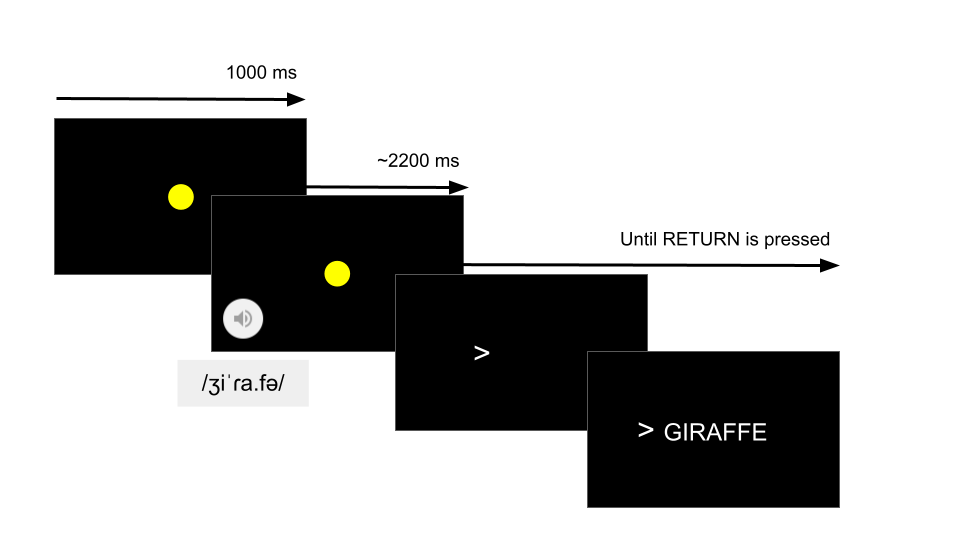
\includegraphics[width=0.8\textwidth,height=\textheight]{../img/design.png}

}

\caption{Schematic representation of a trial in the experimental task.}

\end{figure}%

\subsubsection{Data analysis}\label{data-analysis}

Responses given by English participants to Catalan presented words were
5.35 characters long on average (\emph{Median} = 5, \emph{SD} = 1.79,
Range = 1-14), while their translations to Spanish responses were 5.57
characters long on average (\emph{Median} = 5, \emph{SD} = 1.97, Range =
2-21).

\captionsetup{labelsep=none}

\begin{longtable}{l|rrrr}

\caption{\label{tbl-results}}

\tabularnewline

\toprule
\multicolumn{1}{l}{} & \multicolumn{2}{c}{Correct responses} & \multicolumn{2}{c}{Incorrect responses} \\ 
\cmidrule(lr){2-3} \cmidrule(lr){4-5}
\multicolumn{1}{l}{} & Correct & Typo & Wrong translation & False friend \\ 
\midrule\addlinespace[2.5pt]
\multicolumn{5}{l}{Experiment 1} \\ 
\midrule\addlinespace[2.5pt]
cat-ENG & $429$ ($16.47\%$) & $11$ ($0.42\%$) & $2,082$ ($79.95\%$) & $82$ ($3.15\%$) \\ 
spa-ENG & $374$ ($14.37\%$) & $2$ ($0.08\%$) & $2,117$ ($81.36\%$) & $109$ ($4.19\%$) \\ 
\midrule\addlinespace[2.5pt]
\multicolumn{5}{l}{Experiment 2} \\ 
\midrule\addlinespace[2.5pt]
cat-ENG & $505$ ($18.41\%$) & $7$ ($0.26\%$) & $2,052$ ($74.81\%$) & $179$ ($6.53\%$) \\ 
spa-ENG & $630$ ($20.03\%$) & $6$ ($0.19\%$) & $2,352$ ($74.79\%$) & $157$ ($4.99\%$) \\ 
\midrule\addlinespace[2.5pt]
\multicolumn{5}{l}{Experiment 3} \\ 
\midrule\addlinespace[2.5pt]
cat-SPA & $780$ ($46.93\%$) & $20$ ($1.20\%$) & $736$ ($44.28\%$) & $126$ ($7.58\%$) \\ 
\bottomrule

\end{longtable}

We modelled the probability of participants guessing the correct
translation of each presented word using a generalised multilevel
Bayesian regression model with a Bernoulli logit link distribution. We
included as fixed effects the intercept, the main effects of
\emph{Frequency}, \emph{Cognateness}, and \emph{CLPN}, and the two-way
interaction between \emph{Cognateness} and \emph{CLPN}. We also included
participant-level random intercepts and slopes for the the main effects
and the interaction. \textbf{?@eq-model} shows a formal description of
the model.

To test the practical relevance of each predictor we followed
(\citeproc{ref-krushke2018bayesian}{\textbf{krushke2018bayesian?}}). We
first specified a region of practical equivalence (\emph{ROPE}) around
zero. This area indicates the values of the regression coefficients that
we considered as equivalent to zero. We then computed the 95\% posterior
credible intervals (CrI) of the regression coefficients of interest.
Finally, we calculated the proportion of the 95\% CrI that fell inside
the ROPE. This proportion indicates the probability that the true value
of the coefficient is equivalent to zero.

All analyses were performed in R environment
(\citeproc{ref-rcore2019r}{RCore, 2019}). We used the tidyverse family
of R packages (\citeproc{ref-wickham2019tidyverse}{Wickham et al.,
2019}) to process data and to generate figures. We used the
\texttt{brms} R package (\citeproc{ref-burkner2017brms}{Bürkner, 2017})
using the \texttt{cmdstanr} back-end to the Stan probabilistic language
(\citeproc{ref-carpenter2017stan}{Carpenter et al., 2017}) to estimate
and compare the models (see Appendix 1 for mode details on the models).

\subsection{Results}\label{results}

\textbf{?@tbl-results-1} shows a summary of participants' accuracy
across Experiments 1, 2, and 3. Overall, participants responded less
accurately to words with more CLPNs than to words with fewer CLPNs,
regardless of the amount of phonological similarity between the
presented word and its translation. This is indicated by the size of the
regression coefficient of the two-way interaction between
\emph{Cognateness} and \emph{CLPN} (\(\beta\) = -0.629, 95\% CrI =
{[}-0.982, -0.344{]}, \emph{p}(ROPE) = 0). As anticipated, participants'
performance benefited from an increase in \emph{Cognateness} (\(\beta\)
= 7.11, 95\% CrI = {[}6.567, 7.635{]}, \emph{p}(ROPE) = 0), while the
number of \emph{CLND} had the opposite effect (\(\beta\) = 0.007, 95\%
CrI = {[}-0.107, 0.103{]}, \emph{p}(ROPE) = 0.927). A model including
\emph{Group} as a main effect did not improve the predictive performance
of the model (\(\Delta_{ELPD}\) = -1.33, \(SE\) = 1.14), indicating that
participants in both groups performed equivalently.
Figure~\ref{fig-epreds-1} illustrates the posterior of the average
predictions of the model for words with different values of
\emph{Cognateness} and \emph{CLPN}.

\captionsetup{labelsep=none}

\begin{longtable}{l|rrrrrrr}

\caption{\label{tbl-dataset}}

\tabularnewline

\toprule
\multicolumn{1}{l}{} &  & \multicolumn{3}{c}{Valid trials} & \multicolumn{3}{c}{Accuracy (\%)} \\ 
\cmidrule(lr){3-5} \cmidrule(lr){6-8}
\multicolumn{1}{l}{} & N & Mean ± SD & N trials & Range & Mean ± SD & SE & Range \\ 
\midrule\addlinespace[2.5pt]
\multicolumn{8}{l}{Experiment 1} \\ 
\midrule\addlinespace[2.5pt]
spa-ENG & $27$ & $96.37$ ± $2.88$ ± $2.88$ & $2,602$ & $87$–$98$ & $15.86$ ± $5.20$ & $3.05$ & $8.82$–$28.71$ \\ 
cat-ENG & $32$ & $81.38$ ± $3.17$ ± $3.17$ & $2,604$ & $71$–$83$ & $18.48$ ± $4.89$ & $3.27$ & $10.84$–$32.56$ \\ 
\midrule\addlinespace[2.5pt]
\multicolumn{8}{l}{Experiment 2} \\ 
\midrule\addlinespace[2.5pt]
spa-ENG & $31$ & $101.45$ ± $1.80$ ± $1.80$ & $3,145$ & $92$–$102$ & $21.35$ ± $8.10$ & $3.83$ & $6.60$–$44.34$ \\ 
cat-ENG & $32$ & $85.72$ ± $0.52$ ± $0.52$ & $2,743$ & $84$–$86$ & $20.06$ ± $5.37$ & $3.55$ & $10.00$–$30.00$ \\ 
\midrule\addlinespace[2.5pt]
\multicolumn{8}{l}{Experiment 3} \\ 
\midrule\addlinespace[2.5pt]
cat-SPA & $21$ & $79.14$ ± $3.14$ ± $3.14$ & $1,662$ & $72$–$82$ & $48.30$ ± $5.29$ & $10.54$ & $38.27$–$58.97$ \\ 
\bottomrule

\end{longtable}

\begin{figure}

\centering{

\captionsetup{labelsep=none}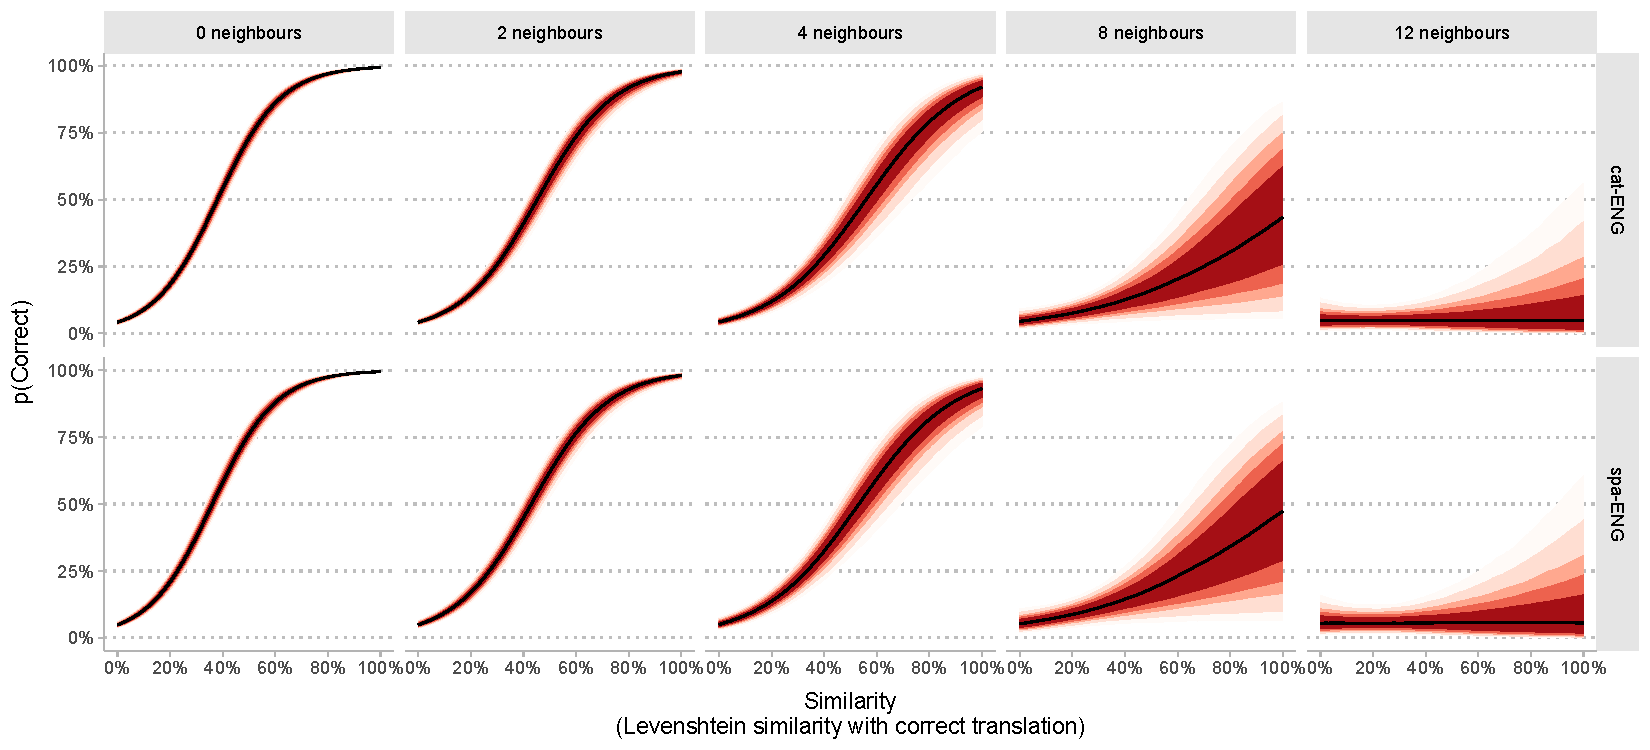
\includegraphics{manuscript_files/figure-pdf/fig-epreds-1-1.pdf}

}

\caption{\label{fig-epreds-1}}

\end{figure}%

\subsection{Discussion}\label{discussion}

\section{Experiment 2}\label{experiment-2}

\subsection{Methods}\label{methods-1}

\subsection{Results}\label{results-1}

\textbf{?@tbl-results-1} shows a summary of participants' accuracy
across Experiments 1, 2, and 3. Overall, participants responded less
accurately to words with more CLPNs than to words with fewer CLPNs,
regardless of the amount of phonological similarity between the
presented word and its translation. This is indicated by the size of the
regression coefficient of the two-way interaction between
\emph{Cognateness} and \emph{CLPN} (\(\beta\) = -0.584, 95\% CrI =
{[}-0.852, -0.331{]}, \emph{p}(ROPE) = 0). As anticipated, participants'
performance benefited from an increase in \emph{Cognateness} (\(\beta\)
= 6.926, 95\% CrI = {[}6.4, 7.461{]}, \emph{p}(ROPE) = 0), while the
number of \emph{CLND} had the opposite effect (\(\beta\) = 0, 95\% CrI =
{[}-0.113, 0.085{]}, \emph{p}(ROPE) = 0.95). A model including
\emph{Group} as a main effect did not improve the predictive performance
of the model (\(\Delta_{ELPD}\) = -6.56, \(SE\) = 3.21), indicating that
participants in both groups performed equivalently.
Figure~\ref{fig-epreds-1} illustrates the posterior of the average
predictions of the model for words with different values of
\emph{Cognateness} and \emph{CLPN}.

\begin{figure}

\centering{

\captionsetup{labelsep=none}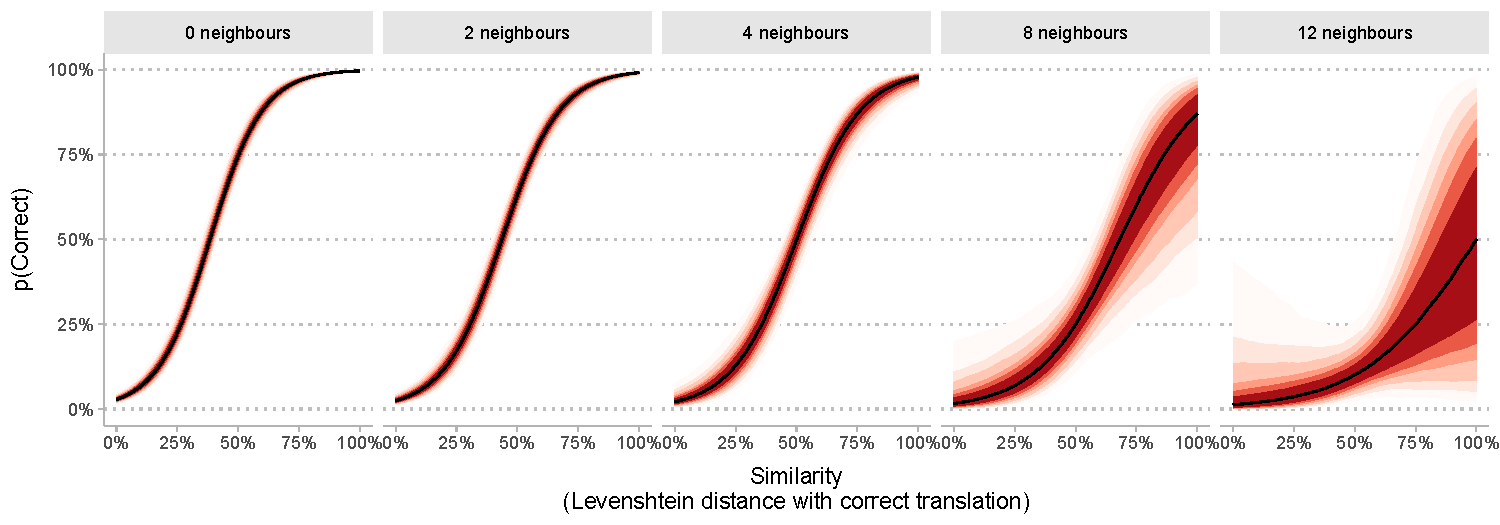
\includegraphics{manuscript_files/figure-pdf/fig-epreds-2-1.pdf}

}

\caption{\label{fig-epreds-2}}

\end{figure}%

\subsection{Discussion}\label{discussion-1}

\section{Experiment 3}\label{experiment-3}

\subsection{Methods}\label{methods-2}

Same as in Experiment 1.

\subsection{Results}\label{results-2}

\textbf{?@tbl-results-1} shows a summary of participants' accuracy
across Experiments 1, 2, and 3. Overall, participants responded less
accurately to words with more CLPNs than to words with fewer CLPNs,
regardless of the amount of phonological similarity between the
presented word and its translation. This is indicated by the size of the
regression coefficient of the two-way interaction between
\emph{Cognateness} and \emph{CLPN} (\(\beta\) = -0.409, 95\% CrI =
{[}-0.895, 0.111{]}, \emph{p}(ROPE) = 0.081). As anticipated,
participants' performance benefited from an increase in
\emph{Cognateness} (\(\beta\) = 9.274, 95\% CrI = {[}8.473, 10.269{]},
\emph{p}(ROPE) = 0), while the number of \emph{CLND} had the opposite
effect (\(\beta\) = -0.069, 95\% CrI = {[}-0.353, 0.192{]},
\emph{p}(ROPE) = 0.492). Figure~\ref{fig-epreds-1} illustrates the
posterior of the average predictions of the model for words with
different values of \emph{Cognateness} and \emph{CLPN}.

\begin{figure}

\centering{

\captionsetup{labelsep=none}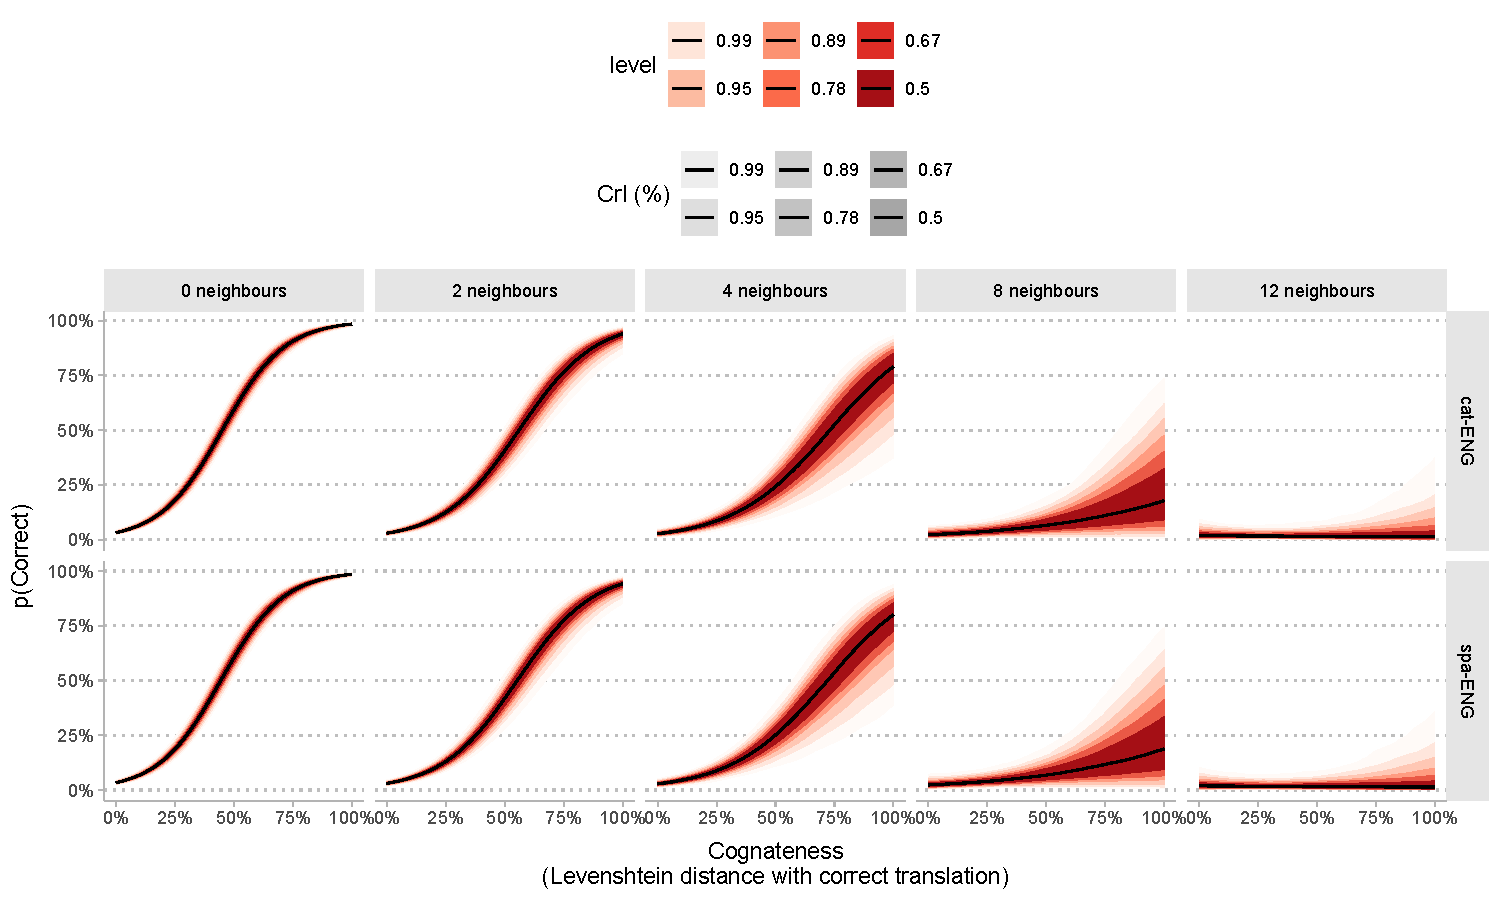
\includegraphics{manuscript_files/figure-pdf/fig-epreds-3-1.pdf}

}

\caption{\label{fig-epreds-3}}

\end{figure}%

\subsection{Discussion}\label{discussion-2}

\section{References}\label{references}

\phantomsection\label{refs}
\begin{CSLReferences}{1}{0}
\bibitem[\citeproctext]{ref-andras2022cognate}
Andras, F., Rivera, M., Bajo, T., Dussias, P. E., \& Paolieri, D.
(2022). Cognate facilitation effect during auditory comprehension of a
second language: A visual world eye-tracking study. \emph{International
Journal of Bilingualism}, 13670069211033359.

\bibitem[\citeproctext]{ref-best2001discrimination}
Best, C. T., McRoberts, G. W., \& Goodell, E. (2001). Discrimination of
non-native consonant contrasts varying in perceptual assimilation to the
listener's native phonological system. \emph{The Journal of the
Acoustical Society of America}, \emph{109}(2), 775--794.

\bibitem[\citeproctext]{ref-broersma2021praat}
Broersma, P., \& Weenink, D. (2021). \emph{Praat: Doing phonetics by
computer {[}computer program{]}} (Version 6.1.54).
\url{http://www.praat.org/}

\bibitem[\citeproctext]{ref-burkner2017brms}
Bürkner, P.-C. (2017). Brms: An r package for bayesian multilevel models
using stan. \emph{Journal of Statistical Software}, \emph{80}(1), 1--28.

\bibitem[\citeproctext]{ref-carpenter2017stan}
Carpenter, B., Gelman, A., Hoffman, M. D., Lee, D., Goodrich, B.,
Betancourt, M., Brubaker, M. A., Guo, J., Li, P., \& Riddell, A. (2017).
Stan: A probabilistic programming language. \emph{Grantee Submission},
\emph{76}(1), 1--32.

\bibitem[\citeproctext]{ref-chen1989patterns}
Chen, H.-C., \& Leung, Y.-S. (1989). Patterns of lexical processing in a
nonnative language. \emph{Journal of Experimental Psychology: Learning,
Memory, and Cognition}, \emph{15}(2), 316.

\bibitem[\citeproctext]{ref-christoffels2006memory}
Christoffels, I. K., De Groot, A. M., \& Kroll, J. F. (2006). Memory and
language skills in simultaneous interpreters: The role of expertise and
language proficiency. \emph{Journal of Memory and Language},
\emph{54}(3), 324--345.

\bibitem[\citeproctext]{ref-costa2000cognate}
Costa, A., Caramazza, A., \& Sebastian-Galles, N. (2000). The cognate
facilitation effect: Implications for models of lexical access.
\emph{Journal of Experimental Psychology: Learning, Memory, and
Cognition}, \emph{26}(5), 1283.

\bibitem[\citeproctext]{ref-cutler2004patterns}
Cutler, A., Weber, A., Smits, R., \& Cooper, N. (2004). Patterns of
english phoneme confusions by native and non-native listeners. \emph{The
Journal of the Acoustical Society of America}, \emph{116}(6),
3668--3678.

\bibitem[\citeproctext]{ref-de2000hard}
De Groot, A. M., \& Keijzer, R. (2000). What is hard to learn is easy to
forget: The roles of word concreteness, cognate status, and word
frequency in foreign-language vocabulary learning and forgetting.
\emph{Language Learning}, \emph{50}(1), 1--56.

\bibitem[\citeproctext]{ref-desroches2022dynamics}
Desroches, A. S., Friesen, D. C., Teles, M., Korade, C. A., \& Forest,
E. W. (2022). The dynamics of spoken word recognition in bilinguals.
\emph{Bilingualism: Language and Cognition}, \emph{25}(4), 705--710.

\bibitem[\citeproctext]{ref-dijkstra2002architecture}
Dijkstra, T., \& Van Heuven, W. J. (2002). The architecture of the
bilingual word recognition system: From identification to decision.
\emph{Bilingualism: Language and Cognition}, \emph{5}(3), 175--197.

\bibitem[\citeproctext]{ref-dufour2003lexical}
Dufour, S., \& Peereman, R. (2003). Lexical competition in phonological
priming: Assessing the role of phonological match and mismatch lengths
between primes and targets. \emph{Memory \& Cognition}, \emph{31},
1271--1283.

\bibitem[\citeproctext]{ref-elias2022cross}
Elias, M., \& Degani, T. (2022). Cross-language interactions during
novel word learning: The contribution of form similarity and participant
characteristics. \emph{Bilingualism: Language and Cognition}, 1--18.

\bibitem[\citeproctext]{ref-goldinger1989priming}
Goldinger, S. D., Luce, P. A., \& Pisoni, D. B. (1989). Priming lexical
neighbors of spoken words: Effects of competition and inhibition.
\emph{Journal of Memory and Language}, \emph{28}(5), 501--518.

\bibitem[\citeproctext]{ref-de1992determinants}
Groot, A. M. de. (1992). Determinants of word translation. \emph{Journal
of Experimental Psychology: Learning, Memory, and Cognition},
\emph{18}(5), 1001.

\bibitem[\citeproctext]{ref-degroot1994forward}
Groot, A. M. de, Dannenburg, L., \& Vanhell, J. G. (1994). Forward and
backward word translation by bilinguals. \emph{Journal of Memory and
Language}, \emph{33}(5), 600--629.

\bibitem[\citeproctext]{ref-hamburger1996phonological}
Hamburger, M., \& Slowiaczek, L. M. (1996). Phonological priming
reflects lexical competition. \emph{Psychonomic Bulletin \& Review},
\emph{3}(4), 520--525.

\bibitem[\citeproctext]{ref-kroll1994category}
Kroll, J. F., \& Stewart, E. (1994). Category interference in
translation and picture naming: Evidence for asymmetric connections
between bilingual memory representations. \emph{Journal of Memory and
Language}, \emph{33}(2), 149--174.

\bibitem[\citeproctext]{ref-lecumberri2010non}
Lecumberri, M. L. G., Cooke, M., \& Cutler, A. (2010). Non-native speech
perception in adverse conditions: A review. \emph{Speech Communication},
\emph{52}(11-12), 864--886.

\bibitem[\citeproctext]{ref-levenshtein1966binary}
Levenshtein, V. I. et al. (1966). Binary codes capable of correcting
deletions, insertions, and reversals. \emph{Soviet Physics Doklady},
\emph{10}, 707--710.

\bibitem[\citeproctext]{ref-lotto1998effects}
Lotto, L., \& De Groot, A. M. (1998). Effects of learning method and
word type on acquiring vocabulary in an unfamiliar language.
\emph{Language Learning}, \emph{48}(1), 31--69.

\bibitem[\citeproctext]{ref-luce1998recognizing}
Luce, P. A., \& Pisoni, D. B. (1998). Recognizing spoken words: The
neighborhood activation model. \emph{Ear and Hearing}, \emph{19}(1), 1.

\bibitem[\citeproctext]{ref-luce1990similarity}
Luce, P. A., Pisoni, D. B., \& Goldinger, S. D. (1990). \emph{Similarity
neighborhoods of spoken words.}

\bibitem[\citeproctext]{ref-marian2012clearpond}
Marian, V., Bartolotti, J., Chabal, S., \& Shook, A. (2012).
\emph{CLEARPOND: Cross-linguistic easy-access resource for phonological
and orthographic neighborhood densities}.

\bibitem[\citeproctext]{ref-mcclelland1981interactive}
McClelland, J. L., \& Rumelhart, D. E. (1981). An interactive activation
model of context effects in letter perception: I. An account of basic
findings. \emph{Psychological Review}, \emph{88}(5), 375.

\bibitem[\citeproctext]{ref-meyer2007activation}
Meyer, A. S., \& Damian, M. F. (2007). Activation of distractor names in
the picture-picture interference paradigm. \emph{Memory \& Cognition},
\emph{35}(3), 494--503.

\bibitem[\citeproctext]{ref-midgley2011effects}
Midgley, K. J., Holcomb, P. J., \& Grainger, J. (2011). Effects of
cognate status on word comprehension in second language learners: An ERP
investigation. \emph{Journal of Cognitive Neuroscience}, \emph{23}(7),
1634--1647.

\bibitem[\citeproctext]{ref-peirce2019psychopy2}
Peirce, J., Gray, J. R., Simpson, S., MacAskill, M., Höchenberger, R.,
Sogo, H., Kastman, E., \& Lindeløv, J. K. (2019). PsychoPy2: Experiments
in behavior made easy. \emph{Behavior Research Methods}, \emph{51}(1),
195--203.

\bibitem[\citeproctext]{ref-phillips2006erp}
Phillips, N. A., Klein, D., Mercier, J., \& Boysson, C. de. (2006). ERP
measures of auditory word repetition and translation priming in
bilinguals. \emph{Brain Research}, \emph{1125}(1), 116--131.

\bibitem[\citeproctext]{ref-potter1984lexical}
Potter, M. C., So, K.-F., Von Eckardt, B., \& Feldman, L. B. (1984).
Lexical and conceptual representation in beginning and proficient
bilinguals. \emph{Journal of Verbal Learning and Verbal Behavior},
\emph{23}(1), 23--38.

\bibitem[\citeproctext]{ref-rcore2019r}
RCore, T. (2019). \emph{R: A language and environment for statistical
computing. R foundation for statistical computing, austria}.

\bibitem[\citeproctext]{ref-schepens2012distributions}
Schepens, J., Dijkstra, T., \& Grootjen, F. (2012). Distributions of
cognates in europe as based on levenshtein distance. \emph{Bilingualism:
Language and Cognition}, \emph{15}(1), 157--166.

\bibitem[\citeproctext]{ref-spivey1999cross}
Spivey, M. J., \& Marian, V. (1999). Cross talk between native and
second languages: Partial activation of an irrelevant lexicon.
\emph{Psychological Science}, \emph{10}(3), 281--284.

\bibitem[\citeproctext]{ref-takata1990english}
Takata, Y., \& Nábělek, A. K. (1990). English consonant recognition in
noise and in reverberation by japanese and american listeners. \emph{The
Journal of the Acoustical Society of America}, \emph{88}(2), 663--666.

\bibitem[\citeproctext]{ref-thierry2007brain}
Thierry, G., \& Wu, Y. J. (2007). Brain potentials reveal unconscious
translation during foreign-language comprehension. \emph{Proceedings of
the National Academy of Sciences}, \emph{104}(30), 12530--12535.

\bibitem[\citeproctext]{ref-valente2018does}
Valente, D., Ferré, P., Soares, A., Rato, A., \& Comesaña, M. (2018).
Does phonological overlap of cognate words modulate cognate acquisition
and processing in developing and skilled readers? \emph{Language
Acquisition}, \emph{25}(4), 438--453.

\bibitem[\citeproctext]{ref-van2014stringdist}
van der Loo, M. P. J. (2014). The stringdist package for approximate
string matching. \emph{The {R} {J}ournal}, \emph{6}, 111--122.
\url{https://CRAN.R-project.org/package=stringdist}

\bibitem[\citeproctext]{ref-van1998orthographic}
Van Heuven, W. J., Dijkstra, T., \& Grainger, J. (1998). Orthographic
neighborhood effects in bilingual word recognition. \emph{Journal of
Memory and Language}, \emph{39}(3), 458--483.

\bibitem[\citeproctext]{ref-van2014subtlex}
Van Heuven, W. J., Mandera, P., Keuleers, E., \& Brysbaert, M. (2014).
SUBTLEX-UK: A new and improved word frequency database for british
english. \emph{Quarterly Journal of Experimental Psychology},
\emph{67}(6), 1176--1190.

\bibitem[\citeproctext]{ref-von2012language}
Von Holzen, K., \& Mani, N. (2012). Language nonselective lexical access
in bilingual toddlers. \emph{Journal of Experimental Child Psychology},
\emph{113}(4), 569--586.

\bibitem[\citeproctext]{ref-weber2004lexical}
Weber, A., \& Cutler, A. (2004). Lexical competition in non-native
spoken-word recognition. \emph{Journal of Memory and Language},
\emph{50}(1), 1--25.

\bibitem[\citeproctext]{ref-wickham2019tidyverse}
Wickham, H., Averick, M., Bryan, J., Chang, W., McGowan, L. D.,
François, R., Grolemund, G., Hayes, A., Henry, L., Hester, J., Kuhn, M.,
Pedersen, T. L., Miller, E., Bache, S. M., Müller, K., Ooms, J.,
Robinson, D., Seidel, D. P., Spinu, V., \ldots{} Yutani, H. (2019).
Welcome to the {tidyverse}. \emph{Journal of Open Source Software},
\emph{4}(43), 1686. \url{https://doi.org/10.21105/joss.01686}

\bibitem[\citeproctext]{ref-andras2022cognate}
Andras, F., Rivera, M., Bajo, T., Dussias, P. E., \& Paolieri, D.
(2022). Cognate facilitation effect during auditory comprehension of a
second language: A visual world eye-tracking study. \emph{International
Journal of Bilingualism}, 13670069211033359.

\bibitem[\citeproctext]{ref-best2001discrimination}
Best, C. T., McRoberts, G. W., \& Goodell, E. (2001). Discrimination of
non-native consonant contrasts varying in perceptual assimilation to the
listener's native phonological system. \emph{The Journal of the
Acoustical Society of America}, \emph{109}(2), 775--794.

\bibitem[\citeproctext]{ref-broersma2021praat}
Broersma, P., \& Weenink, D. (2021). \emph{Praat: Doing phonetics by
computer {[}computer program{]}} (Version 6.1.54).
\url{http://www.praat.org/}

\bibitem[\citeproctext]{ref-burkner2017brms}
Bürkner, P.-C. (2017). Brms: An r package for bayesian multilevel models
using stan. \emph{Journal of Statistical Software}, \emph{80}(1), 1--28.

\bibitem[\citeproctext]{ref-carpenter2017stan}
Carpenter, B., Gelman, A., Hoffman, M. D., Lee, D., Goodrich, B.,
Betancourt, M., Brubaker, M. A., Guo, J., Li, P., \& Riddell, A. (2017).
Stan: A probabilistic programming language. \emph{Grantee Submission},
\emph{76}(1), 1--32.

\bibitem[\citeproctext]{ref-chen1989patterns}
Chen, H.-C., \& Leung, Y.-S. (1989). Patterns of lexical processing in a
nonnative language. \emph{Journal of Experimental Psychology: Learning,
Memory, and Cognition}, \emph{15}(2), 316.

\bibitem[\citeproctext]{ref-christoffels2006memory}
Christoffels, I. K., De Groot, A. M., \& Kroll, J. F. (2006). Memory and
language skills in simultaneous interpreters: The role of expertise and
language proficiency. \emph{Journal of Memory and Language},
\emph{54}(3), 324--345.

\bibitem[\citeproctext]{ref-costa2000cognate}
Costa, A., Caramazza, A., \& Sebastian-Galles, N. (2000). The cognate
facilitation effect: Implications for models of lexical access.
\emph{Journal of Experimental Psychology: Learning, Memory, and
Cognition}, \emph{26}(5), 1283.

\bibitem[\citeproctext]{ref-cutler2004patterns}
Cutler, A., Weber, A., Smits, R., \& Cooper, N. (2004). Patterns of
english phoneme confusions by native and non-native listeners. \emph{The
Journal of the Acoustical Society of America}, \emph{116}(6),
3668--3678.

\bibitem[\citeproctext]{ref-de2000hard}
De Groot, A. M., \& Keijzer, R. (2000). What is hard to learn is easy to
forget: The roles of word concreteness, cognate status, and word
frequency in foreign-language vocabulary learning and forgetting.
\emph{Language Learning}, \emph{50}(1), 1--56.

\bibitem[\citeproctext]{ref-desroches2022dynamics}
Desroches, A. S., Friesen, D. C., Teles, M., Korade, C. A., \& Forest,
E. W. (2022). The dynamics of spoken word recognition in bilinguals.
\emph{Bilingualism: Language and Cognition}, \emph{25}(4), 705--710.

\bibitem[\citeproctext]{ref-dijkstra2002architecture}
Dijkstra, T., \& Van Heuven, W. J. (2002). The architecture of the
bilingual word recognition system: From identification to decision.
\emph{Bilingualism: Language and Cognition}, \emph{5}(3), 175--197.

\bibitem[\citeproctext]{ref-dufour2003lexical}
Dufour, S., \& Peereman, R. (2003). Lexical competition in phonological
priming: Assessing the role of phonological match and mismatch lengths
between primes and targets. \emph{Memory \& Cognition}, \emph{31},
1271--1283.

\bibitem[\citeproctext]{ref-elias2022cross}
Elias, M., \& Degani, T. (2022). Cross-language interactions during
novel word learning: The contribution of form similarity and participant
characteristics. \emph{Bilingualism: Language and Cognition}, 1--18.

\bibitem[\citeproctext]{ref-goldinger1989priming}
Goldinger, S. D., Luce, P. A., \& Pisoni, D. B. (1989). Priming lexical
neighbors of spoken words: Effects of competition and inhibition.
\emph{Journal of Memory and Language}, \emph{28}(5), 501--518.

\bibitem[\citeproctext]{ref-de1992determinants}
Groot, A. M. de. (1992). Determinants of word translation. \emph{Journal
of Experimental Psychology: Learning, Memory, and Cognition},
\emph{18}(5), 1001.

\bibitem[\citeproctext]{ref-degroot1994forward}
Groot, A. M. de, Dannenburg, L., \& Vanhell, J. G. (1994). Forward and
backward word translation by bilinguals. \emph{Journal of Memory and
Language}, \emph{33}(5), 600--629.

\bibitem[\citeproctext]{ref-hamburger1996phonological}
Hamburger, M., \& Slowiaczek, L. M. (1996). Phonological priming
reflects lexical competition. \emph{Psychonomic Bulletin \& Review},
\emph{3}(4), 520--525.

\bibitem[\citeproctext]{ref-kroll1994category}
Kroll, J. F., \& Stewart, E. (1994). Category interference in
translation and picture naming: Evidence for asymmetric connections
between bilingual memory representations. \emph{Journal of Memory and
Language}, \emph{33}(2), 149--174.

\bibitem[\citeproctext]{ref-lecumberri2010non}
Lecumberri, M. L. G., Cooke, M., \& Cutler, A. (2010). Non-native speech
perception in adverse conditions: A review. \emph{Speech Communication},
\emph{52}(11-12), 864--886.

\bibitem[\citeproctext]{ref-levenshtein1966binary}
Levenshtein, V. I. et al. (1966). Binary codes capable of correcting
deletions, insertions, and reversals. \emph{Soviet Physics Doklady},
\emph{10}, 707--710.

\bibitem[\citeproctext]{ref-lotto1998effects}
Lotto, L., \& De Groot, A. M. (1998). Effects of learning method and
word type on acquiring vocabulary in an unfamiliar language.
\emph{Language Learning}, \emph{48}(1), 31--69.

\bibitem[\citeproctext]{ref-luce1998recognizing}
Luce, P. A., \& Pisoni, D. B. (1998). Recognizing spoken words: The
neighborhood activation model. \emph{Ear and Hearing}, \emph{19}(1), 1.

\bibitem[\citeproctext]{ref-luce1990similarity}
Luce, P. A., Pisoni, D. B., \& Goldinger, S. D. (1990). \emph{Similarity
neighborhoods of spoken words.}

\bibitem[\citeproctext]{ref-marian2012clearpond}
Marian, V., Bartolotti, J., Chabal, S., \& Shook, A. (2012).
\emph{CLEARPOND: Cross-linguistic easy-access resource for phonological
and orthographic neighborhood densities}.

\bibitem[\citeproctext]{ref-mcclelland1981interactive}
McClelland, J. L., \& Rumelhart, D. E. (1981). An interactive activation
model of context effects in letter perception: I. An account of basic
findings. \emph{Psychological Review}, \emph{88}(5), 375.

\bibitem[\citeproctext]{ref-meyer2007activation}
Meyer, A. S., \& Damian, M. F. (2007). Activation of distractor names in
the picture-picture interference paradigm. \emph{Memory \& Cognition},
\emph{35}(3), 494--503.

\bibitem[\citeproctext]{ref-midgley2011effects}
Midgley, K. J., Holcomb, P. J., \& Grainger, J. (2011). Effects of
cognate status on word comprehension in second language learners: An ERP
investigation. \emph{Journal of Cognitive Neuroscience}, \emph{23}(7),
1634--1647.

\bibitem[\citeproctext]{ref-peirce2019psychopy2}
Peirce, J., Gray, J. R., Simpson, S., MacAskill, M., Höchenberger, R.,
Sogo, H., Kastman, E., \& Lindeløv, J. K. (2019). PsychoPy2: Experiments
in behavior made easy. \emph{Behavior Research Methods}, \emph{51}(1),
195--203.

\bibitem[\citeproctext]{ref-phillips2006erp}
Phillips, N. A., Klein, D., Mercier, J., \& Boysson, C. de. (2006). ERP
measures of auditory word repetition and translation priming in
bilinguals. \emph{Brain Research}, \emph{1125}(1), 116--131.

\bibitem[\citeproctext]{ref-potter1984lexical}
Potter, M. C., So, K.-F., Von Eckardt, B., \& Feldman, L. B. (1984).
Lexical and conceptual representation in beginning and proficient
bilinguals. \emph{Journal of Verbal Learning and Verbal Behavior},
\emph{23}(1), 23--38.

\bibitem[\citeproctext]{ref-rcore2019r}
RCore, T. (2019). \emph{R: A language and environment for statistical
computing. R foundation for statistical computing, austria}.

\bibitem[\citeproctext]{ref-schepens2012distributions}
Schepens, J., Dijkstra, T., \& Grootjen, F. (2012). Distributions of
cognates in europe as based on levenshtein distance. \emph{Bilingualism:
Language and Cognition}, \emph{15}(1), 157--166.

\bibitem[\citeproctext]{ref-spivey1999cross}
Spivey, M. J., \& Marian, V. (1999). Cross talk between native and
second languages: Partial activation of an irrelevant lexicon.
\emph{Psychological Science}, \emph{10}(3), 281--284.

\bibitem[\citeproctext]{ref-takata1990english}
Takata, Y., \& Nábělek, A. K. (1990). English consonant recognition in
noise and in reverberation by japanese and american listeners. \emph{The
Journal of the Acoustical Society of America}, \emph{88}(2), 663--666.

\bibitem[\citeproctext]{ref-thierry2007brain}
Thierry, G., \& Wu, Y. J. (2007). Brain potentials reveal unconscious
translation during foreign-language comprehension. \emph{Proceedings of
the National Academy of Sciences}, \emph{104}(30), 12530--12535.

\bibitem[\citeproctext]{ref-valente2018does}
Valente, D., Ferré, P., Soares, A., Rato, A., \& Comesaña, M. (2018).
Does phonological overlap of cognate words modulate cognate acquisition
and processing in developing and skilled readers? \emph{Language
Acquisition}, \emph{25}(4), 438--453.

\bibitem[\citeproctext]{ref-van2014stringdist}
van der Loo, M. P. J. (2014). The stringdist package for approximate
string matching. \emph{The {R} {J}ournal}, \emph{6}, 111--122.
\url{https://CRAN.R-project.org/package=stringdist}

\bibitem[\citeproctext]{ref-van1998orthographic}
Van Heuven, W. J., Dijkstra, T., \& Grainger, J. (1998). Orthographic
neighborhood effects in bilingual word recognition. \emph{Journal of
Memory and Language}, \emph{39}(3), 458--483.

\bibitem[\citeproctext]{ref-van2014subtlex}
Van Heuven, W. J., Mandera, P., Keuleers, E., \& Brysbaert, M. (2014).
SUBTLEX-UK: A new and improved word frequency database for british
english. \emph{Quarterly Journal of Experimental Psychology},
\emph{67}(6), 1176--1190.

\bibitem[\citeproctext]{ref-von2012language}
Von Holzen, K., \& Mani, N. (2012). Language nonselective lexical access
in bilingual toddlers. \emph{Journal of Experimental Child Psychology},
\emph{113}(4), 569--586.

\bibitem[\citeproctext]{ref-weber2004lexical}
Weber, A., \& Cutler, A. (2004). Lexical competition in non-native
spoken-word recognition. \emph{Journal of Memory and Language},
\emph{50}(1), 1--25.

\bibitem[\citeproctext]{ref-wickham2019tidyverse}
Wickham, H., Averick, M., Bryan, J., Chang, W., McGowan, L. D.,
François, R., Grolemund, G., Hayes, A., Henry, L., Hester, J., Kuhn, M.,
Pedersen, T. L., Miller, E., Bache, S. M., Müller, K., Ooms, J.,
Robinson, D., Seidel, D. P., Spinu, V., \ldots{} Yutani, H. (2019).
Welcome to the {tidyverse}. \emph{Journal of Open Source Software},
\emph{4}(43), 1686. \url{https://doi.org/10.21105/joss.01686}

\end{CSLReferences}



\end{document}
